\documentclass{beamer}
\nonstopmode
\usetheme{Boadilla}
%\usetheme{Madrid}
%\usetheme{Pittsburgh}
%\usetheme{Rochester}
\usecolortheme{beaver}
\usecolortheme{orchid}
\setbeameroption{show notes}
\hypersetup{pdfstartview={Fit}} % fits the presentation to the window when first displayed
\usepackage{xcolor}
\usepackage{adjustbox} %Used to fit tables to slides

\usepackage{array} %used for math mode in table aod
\usepackage{import} % \subimput alows importing of Inkscape pdf+tex files in subfolder

\title[Perception and Working Memory in Neglect]{Perceptual and Working Memory Deficits in Unilateral Neglect}
\subtitle{}

\author{Jason Locklin}
\institute[University of Waterloo]
{Department of Psychology\\
	University of Waterloo\\
	\bigskip
	Supervisor: Dr.\ James Danckert
}
\date[August 6, 2015]
{}% <- QR

\AtBeginSection[]
{\begin{frame}
		\frametitle{Overview}
		\tableofcontents[currentsection]
	\end{frame}
}


\begin{document}

%%%%%%%%%%%%%%%%%%%%%%%% GENERAL INTRODUCTION
\frame{\titlepage}
\section*{}

\begin{frame}
	\frametitle{Unilateral Neglect}
	\begin{columns}
		\begin{column}{0.5\textwidth}
			\begin{itemize}
				\item Typically results from damage to the right inferior parietal or superior temporal cortex.
				\bigskip
				\item Inability to respond to the left side of space.
			\end{itemize}
		\end{column}
		\begin{column}{0.5\textwidth}
			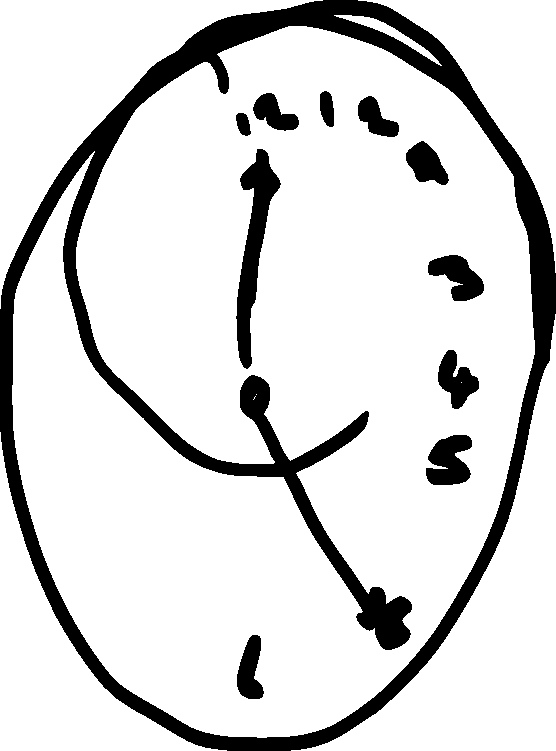
\includegraphics
			[height=.5\textheight,width=\textwidth,keepaspectratio]
			{img/Clock_drawing.pdf}
		\end{column}
	\end{columns}
\end{frame}


\begin{frame}
	\frametitle{Neglect as a Lateralized Disorder of Attention}
	\begin{columns}
		\begin{column}{0.5\textwidth}
			\begin{itemize}
				\item	Preferential orienting rightward
				\bigskip
				\item Delayed re-orienting leftward.
				\bigskip
				\item Limitations
				%\item Evidence from covert orienting and visual search.
				%\item Other non-lateralized deficits of attention such as selective attention (attentional blink), and sustained attention.
			\end{itemize}
		\end{column}
		\begin{column}{0.5\textwidth}
			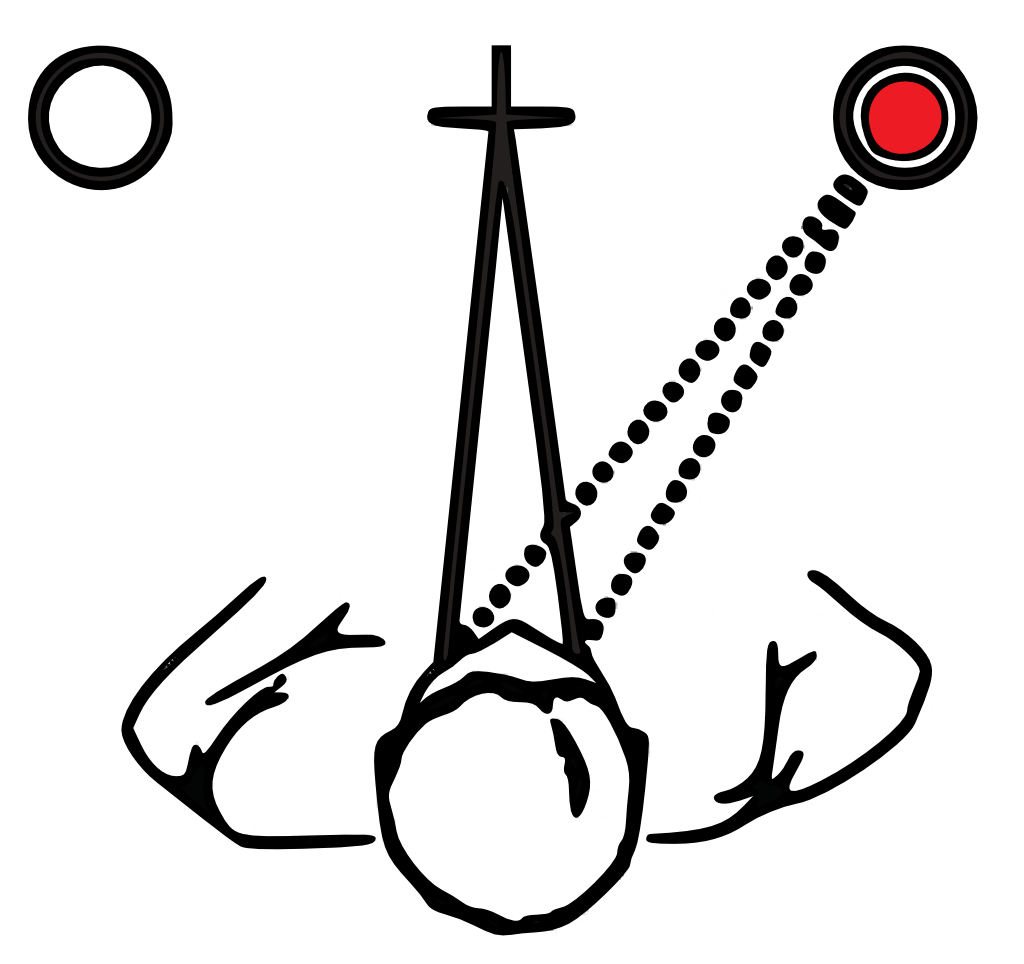
\includegraphics
			[height=.5\textheight,width=\textwidth,keepaspectratio]
			{img/orienting.png}
		\end{column}
	\end{columns}
	\end{frame}



\section[Attention and WM]{Is visual working memory closely coupled to lateralized attention biases?}

%%%% VWM
\subsection*{Visual Working Memory}

\begin{frame}
	\frametitle{Visual Working Memory Task}
	\def\svgwidth{1\textwidth}
	\subimport{VWM/}{VWM/fig_VWM-task.pdf_tex}
\end{frame}

\begin{frame}
	\frametitle{Figure 2.4: Probability of Correct Target Selection}
	\centering
	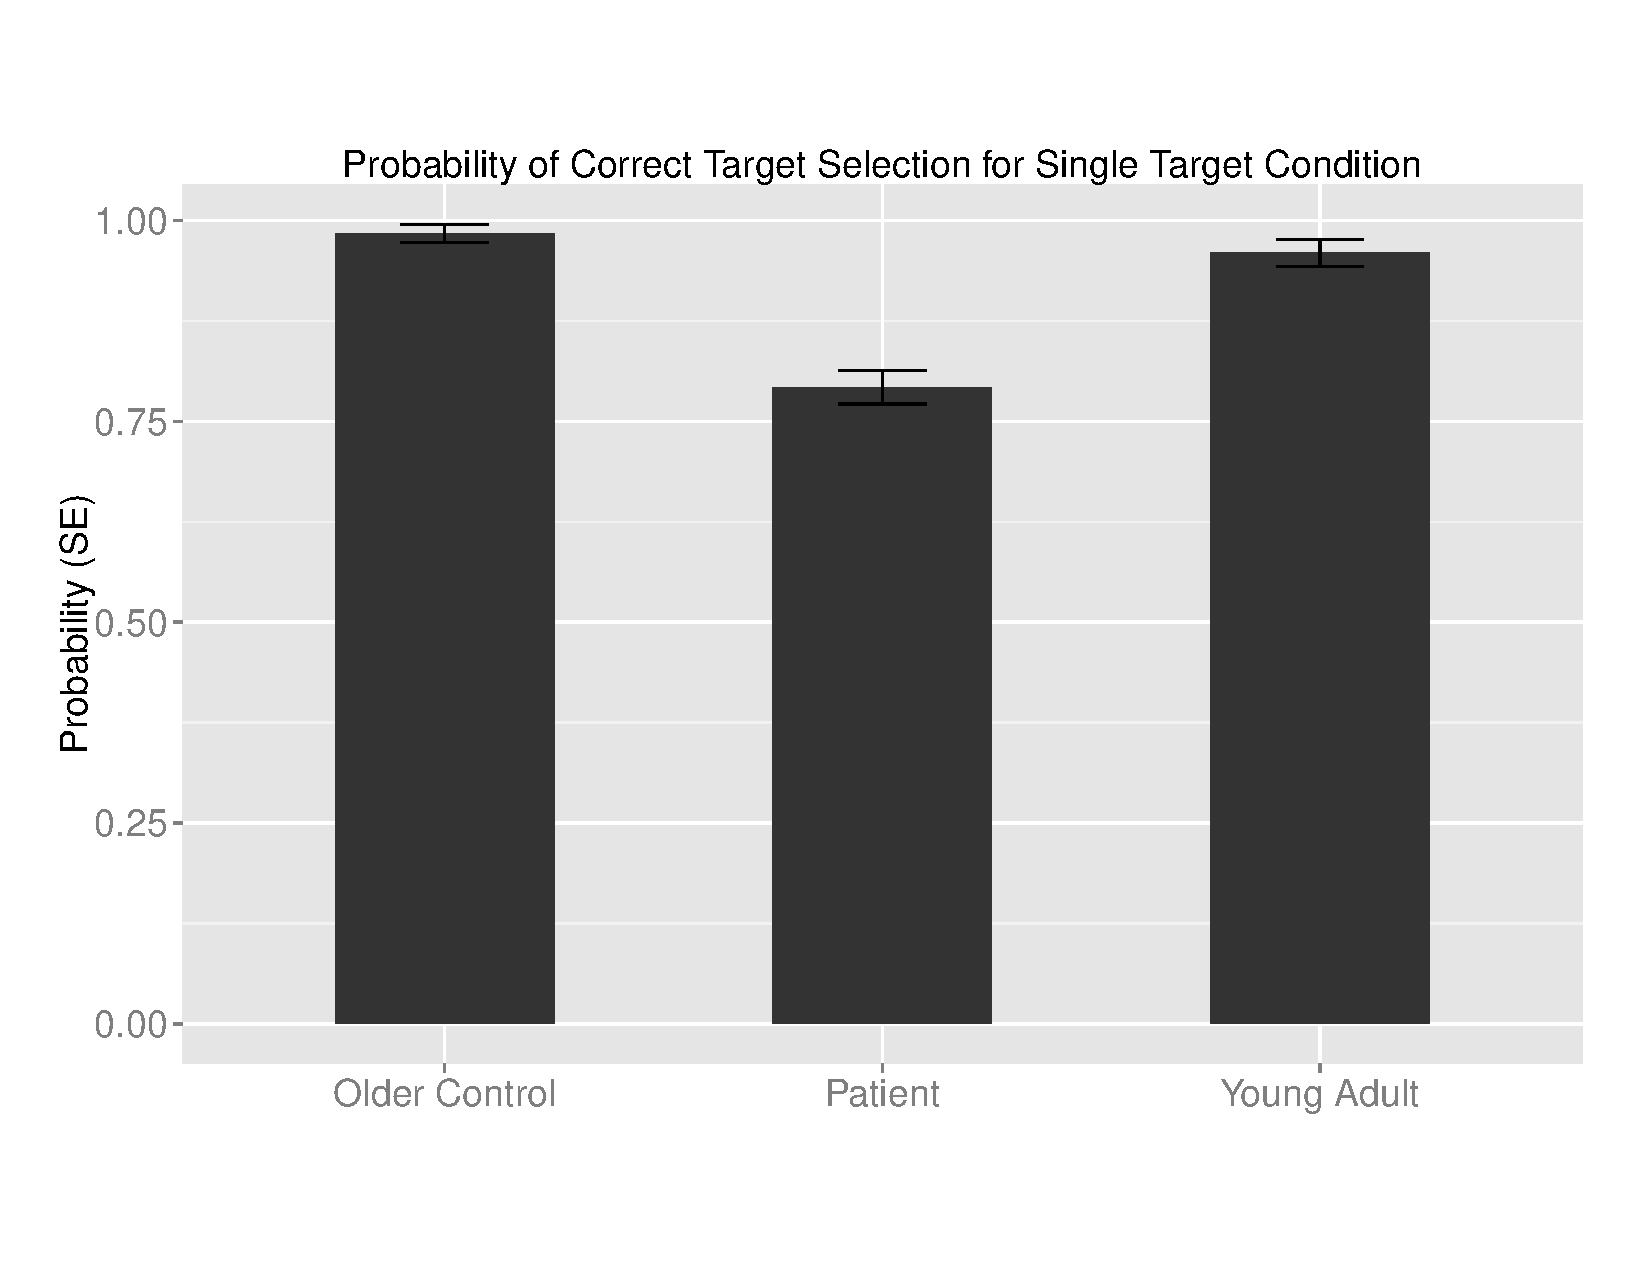
\includegraphics
	[height=.8\textheight,width=\textwidth,keepaspectratio]
	{VWM/fig_VWM_1Target.pdf}
\end{frame}

\begin{frame}
	\frametitle{Figure 2.5: Probability of Non-Target Selection}
	\centering
	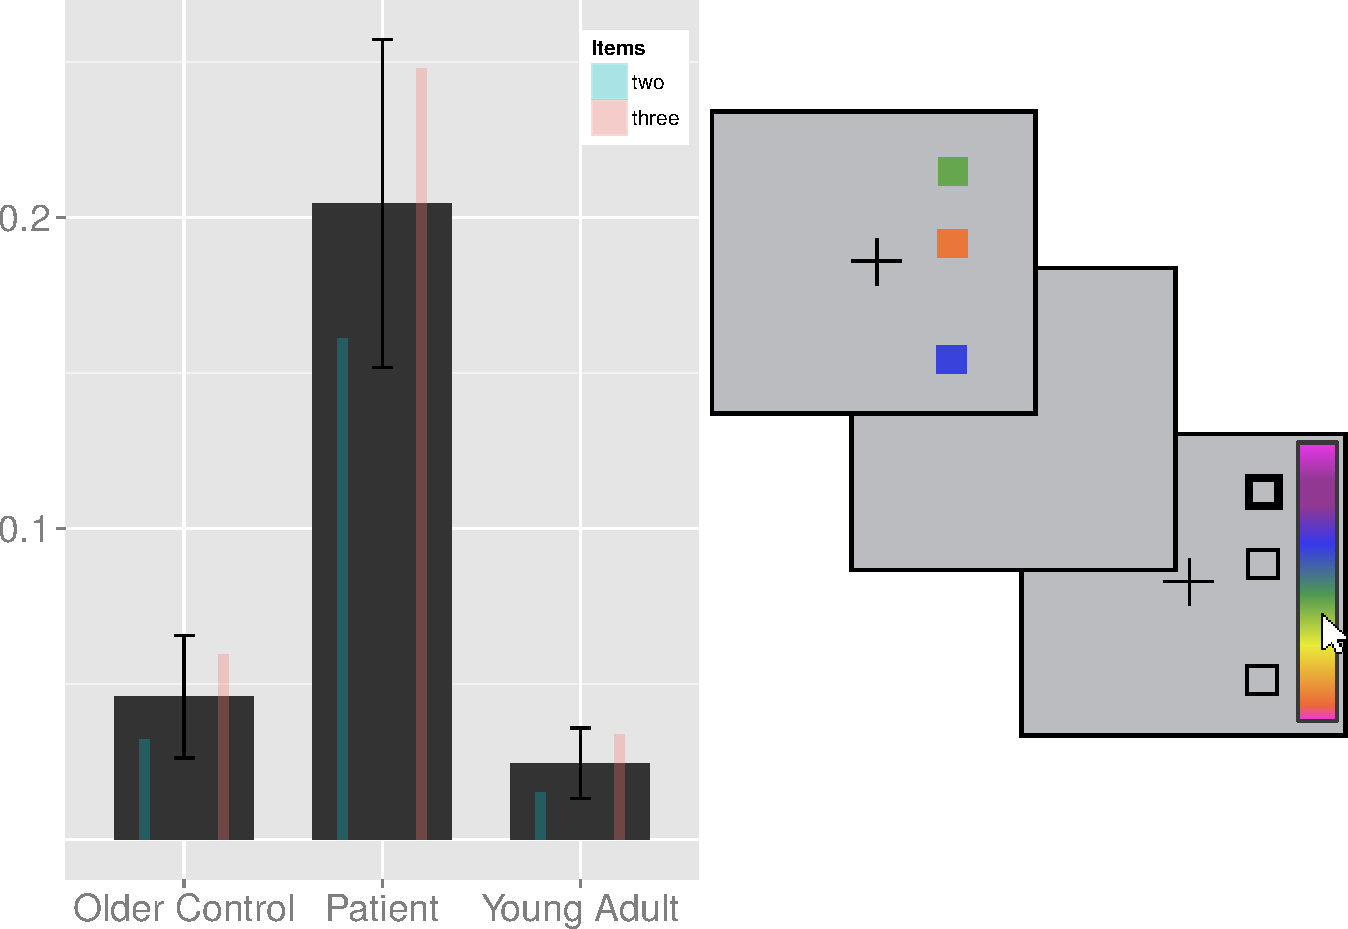
\includegraphics
	[height=.8\textheight,width=\textwidth,keepaspectratio]
	{VWM/fig_VWM_PNT.pdf}
\end{frame}


%%%% COVAT
\subsection*{Covert Orienting}
\begin{frame}
	\frametitle{Covert Orienting Task}
	\def\svgwidth{1\textwidth}
	\subimport{VWM/}{VWM/fig_COVAT-task.pdf_tex}
\end{frame}

\begin{frame}
	\frametitle{Figure 2.6: Patient Leftward Cue Effect Sizes (CES)}
	\centering
	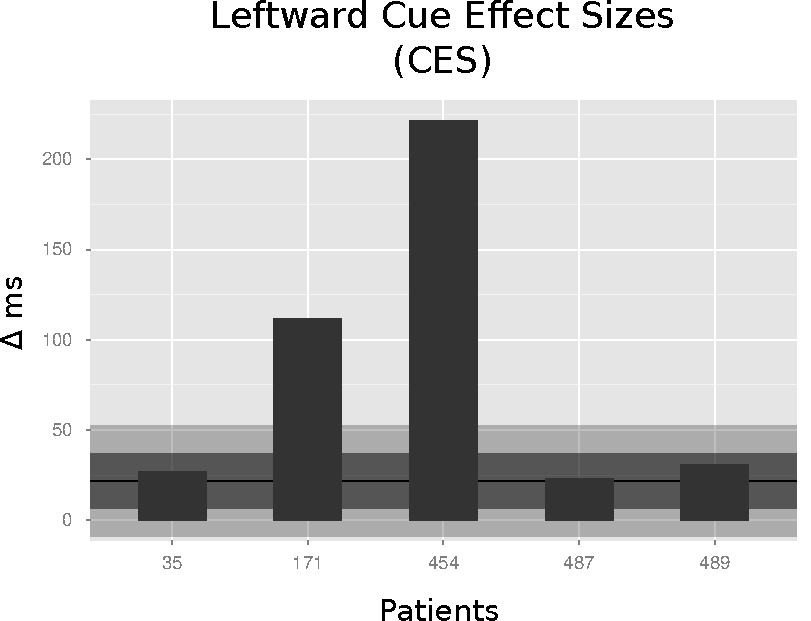
\includegraphics
	[height=.8\textheight,width=\textwidth,keepaspectratio]
	{VWM/fig_COVAT.pdf}
\end{frame}

\subsection*{}

%%%%%%%%%%%%%%%%%%%%%%%% EXPERIMENT TWO
\section[Prisms]{Does treatment of attention deficits with prisms influence perceptual representations?}

\begin{frame}
	\frametitle{Prism Adaptation}
	\begin{columns}
		\begin{column}{0.5\textwidth}
\begin{itemize}
	\item $10^{\circ}$ rightward shifting prisms.
	\item Alternate pointing to left and right table-top targets for 5 minutes.
\end{itemize}
		\end{column}
		\begin{column}{0.5\textwidth}
			\only<1>{ 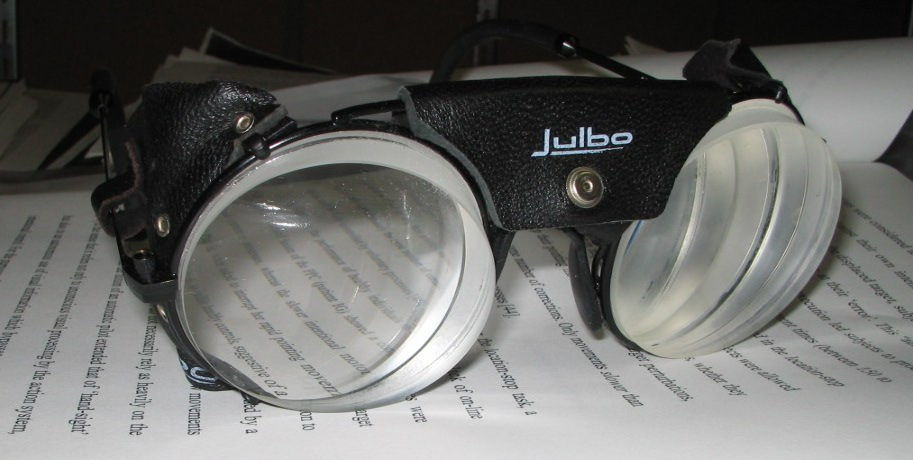
\includegraphics
			[height=.5\textheight,width=\textwidth,keepaspectratio]
			{img/prisms.jpg}}
		\end{column}
	\end{columns}
\end{frame}



%%%% SWM
\subsection*{Spatial Working Memory}

\begin{frame}
	\frametitle{Spatial Working Memory Task}
	\def\svgwidth{0.7\textwidth}
	\subimport{Prisms/}{Prisms/fig_SWM-task.pdf_tex}
\end{frame}

\begin{frame}
	\frametitle{Figure 3.2: Spatial Working Memory}
	\centering
	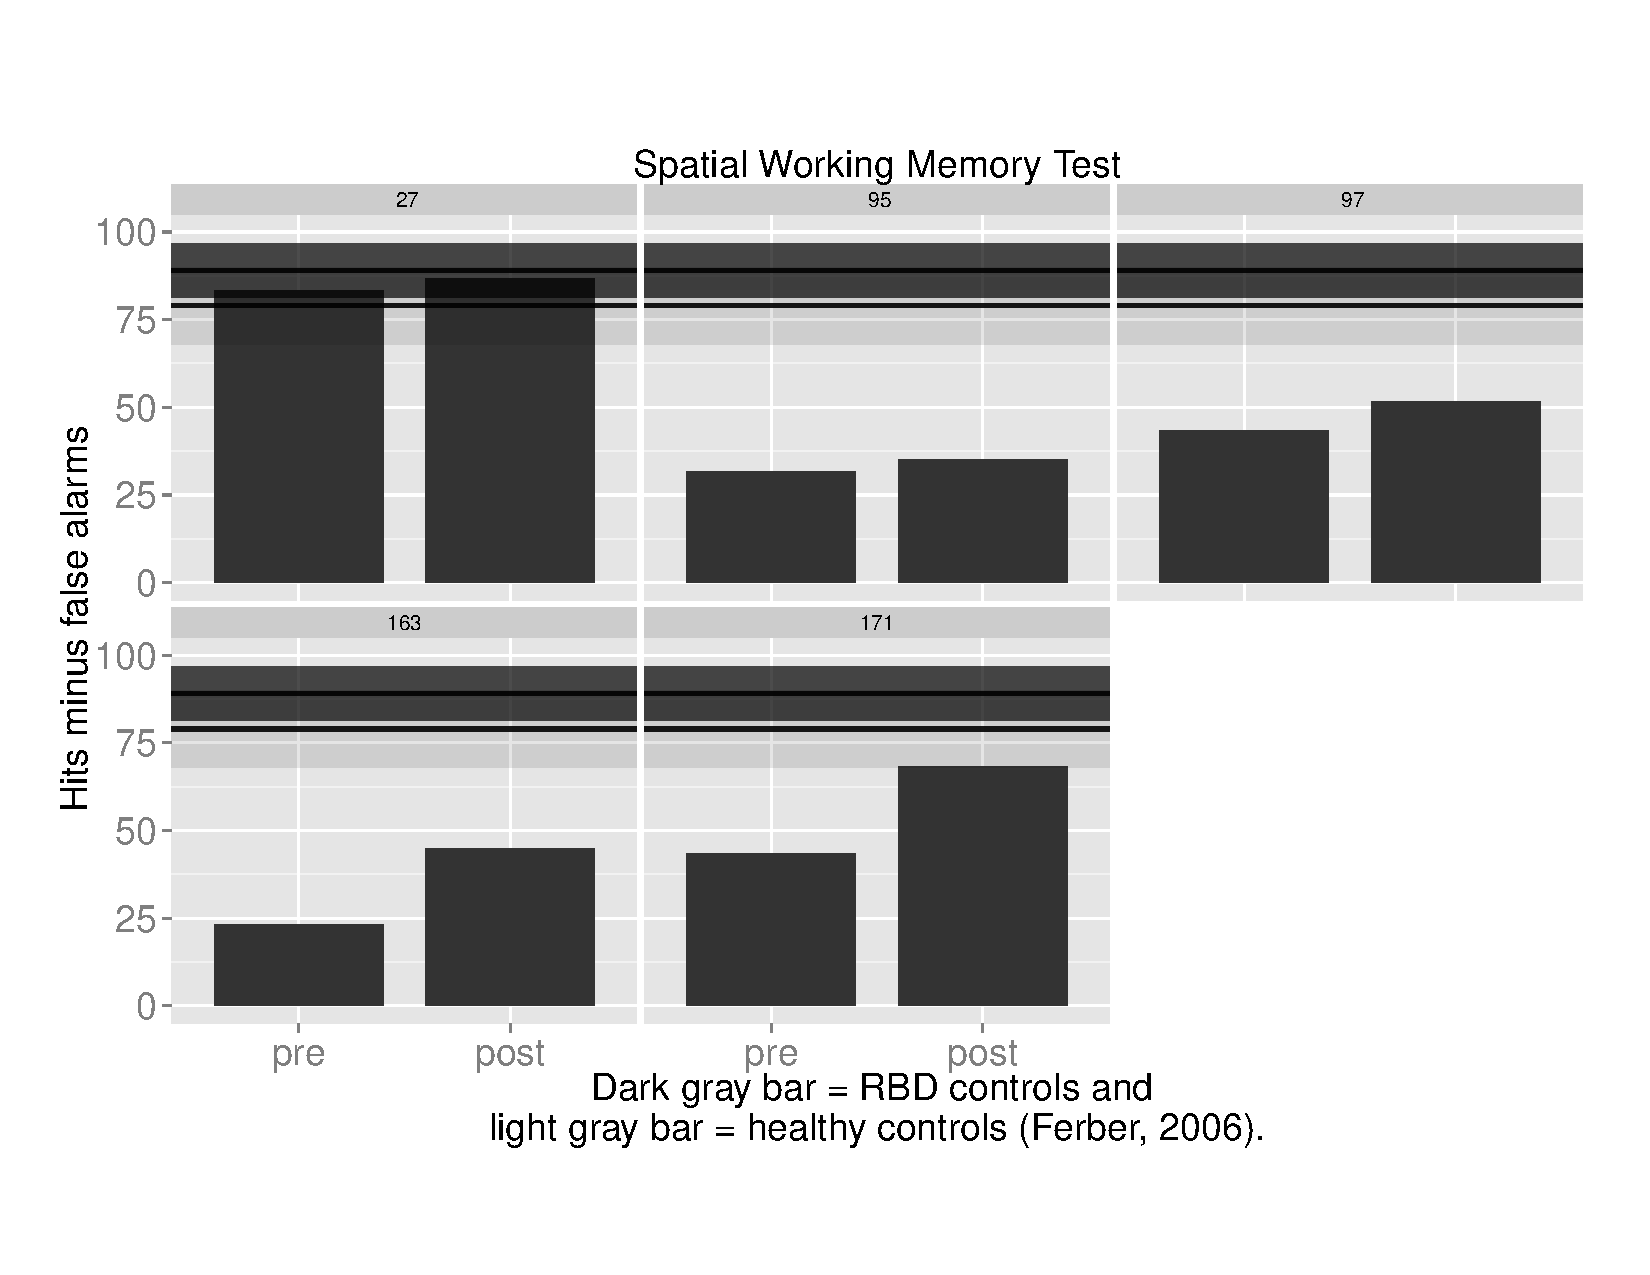
\includegraphics
	[height=.85\textheight,width=\textwidth,keepaspectratio]
	{Prisms/fig_SWM.pdf}
\end{frame}


%%%% TE
\subsection*{Time Perception}
\begin{frame}
	\frametitle{Temporal Estimation Task}
	\def\svgwidth{0.9\textwidth}
	\subimport{Prisms/}{Prisms/fig_TE-task.pdf_tex}
\end{frame}

\begin{frame}
	\frametitle{Figure 3.3: Temporal Estimation Across Intervals}
	\centering
	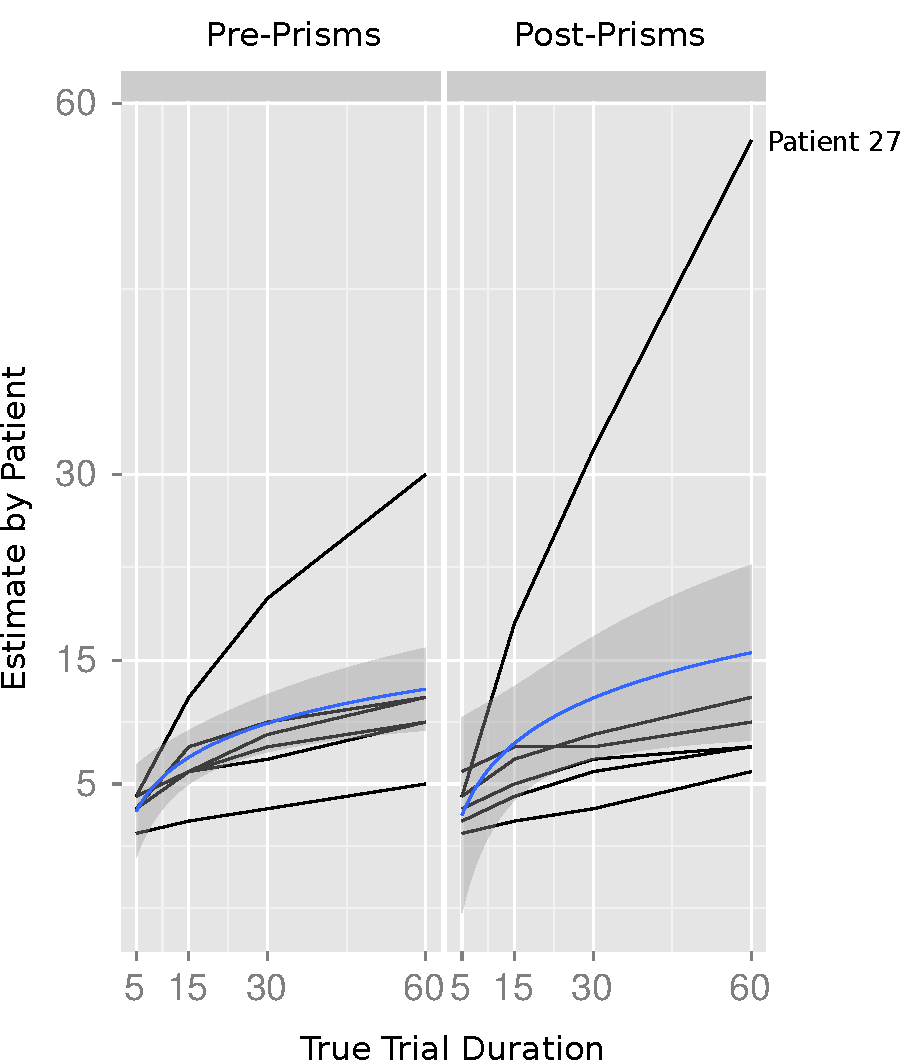
\includegraphics
	[height=.75\textheight,width=\textwidth,keepaspectratio]
	{Prisms/fig_TE_right.pdf}
\end{frame}

%%%%%%%%%%%%%%%%%%%%%%%% EXPERIMENT THREE
\section[Saccadic Adaptation]{Is Saccadic Adaptation capable of influencing perceptual biases\?}


\begin{frame}
	\frametitle{Saccadic Adaptation}
	\centering
	\def\svgwidth{0.7\textwidth}
	\tiny
	\subimport{SA/}{SA/fig_SA_a.pdf_tex}
\end{frame}

\begin{frame}
	\frametitle{Figure 4.4: Effect of Saccadic Adaptation}
	\centering
	\def\svgwidth{0.9\textwidth}
	\tiny
	\subimport{SA/}{SA/fig_Adaptation_allTrials.pdf_tex}
\end{frame}

\begin{frame}
	\frametitle{Landmark Task}
	\def\svgwidth{0.8\textwidth}
	\subimport{SA/}{SA/fig_Landmark-task.pdf_tex}
\end{frame}

\begin{frame}
	\frametitle{Line Bisection Task}
	\def\svgwidth{0.9\textwidth}
	\subimport{SA/}{SA/fig_LineBisection.pdf_tex}
\end{frame}

\begin{frame}
	\frametitle{Impact on Line Bisection (LB) and Landmark Task (LT)}
	\begin{itemize}
		\item No measurable change in either LB or LT post adaptation.
		\item ``Strong adapters'' also showed no change.
	\end{itemize}

\end{frame}


%%%%%%%%%%%%%%%%%%%%%%%% CONCLUDING MATTER
\section*{}
\begin{frame}
	\frametitle{Overall Conclusions}
	\begin{itemize}
		\item WM deficits appear to be independent of lateralized attention deficits in neglect.
		\item Perceptual representations, more generally, may be uninfluenced by changes in those lateralized attention deficits.
		\item More research is needed to examine saccadic adaptation as a possible method to influence those perceptual representations.
	\end{itemize}
\end{frame}

\begin{frame}
	\frametitle{Future Directions}
	\begin{itemize}
		\item Improve saccadic adaptation procedure, possibly with whole-field adaptation
		\item If successful, compare the two in a neglect population.
	\end{itemize}
\end{frame}

\begin{frame}
	\frametitle{Acknowledgements}
	Dr. James Danckert\\
	With funding from the Heart and Stroke Foundation.
\end{frame}


%%%%%%%%%%%%%%%%%%%%%%%% APPENDIX
\subsection*{Appendix}

\begin{frame}[noframenumbering]
	\frametitle{Spatial Working Memory}
	\centering 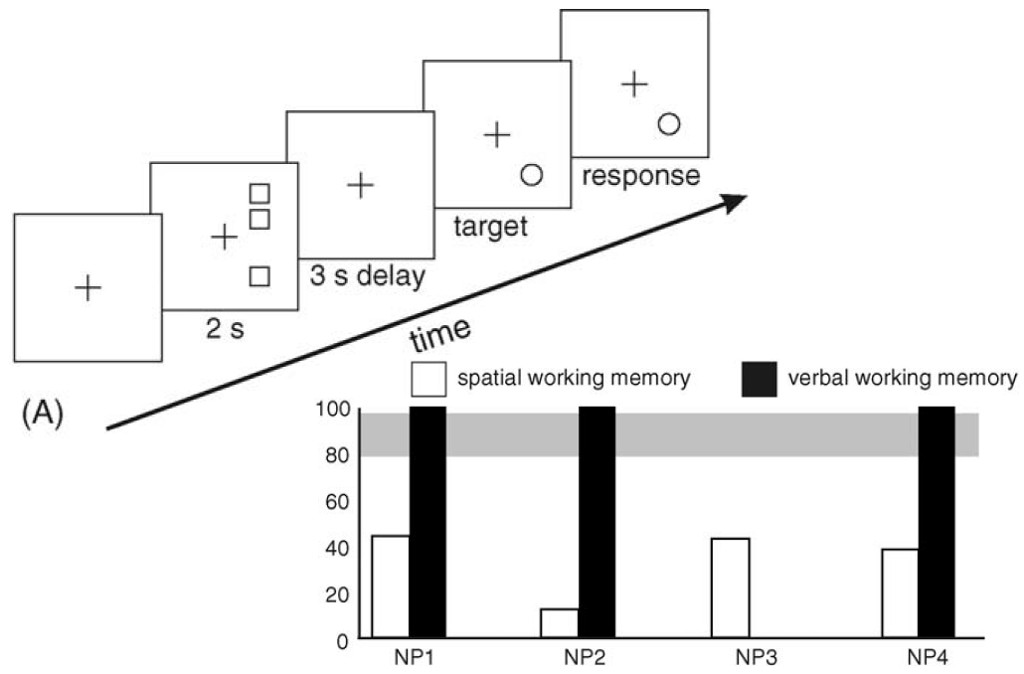
\includegraphics
			[height=.8\textheight,keepaspectratio]
			{img/danckert2006.png}\\
	\tiny (Danckert \& Ferber 2006)
\end{frame}

\begin{frame}[noframenumbering]
	\frametitle{Table 2.1}
	\adjustbox{max height=\dimexpr\textheight-5.5cm\relax,
	max width=\textwidth}{\begin{tabular}{rrllrrrrlr}
  \hline
 & Age & Sex & Handedness & CES & VWM(1) & VWM(2/3) & Stars & Copying & Bisection \\ 
  \hline
487 &  61 & F & Right & 23.0 & 0.15 & 0.04 & 0& + & 2.2 \\ 
  35 &  51 & F & Right & 27.0 & 0.15 & 0.04 & 17& + & 0.1 \\ 
  489 &  66 & M & Left & 31.0 & 0.25 & 0.08 & 0& + & 1.0 \\ 
  171 &  71 & F & Left & 112.0 & 0.13 & 0.00 & 0& -  & 1.4 \\ 
  454 &  70 & M & Right & 221.5 & 0.23 & 0.17 & 0& + & 6.3 \\ 
  213 &  65 & F & Right & NA & 0.2 & 0.30 & 100& + & 7.3 \\ 
  396 &  85 & M & Right & NA & 0.3 & 0.55 & 87& + & 8.1 \\ 
  465 &  63 & F & Right & NA & 0.3 & 0.45 & 97& + & 12.9 \\ 
   \hline
\end{tabular}
}
\end{frame}

\begin{frame}[noframenumbering]
\frametitle{Exp. 1: Participants and Procedure}
\begin{itemize}
	\item 8 RBD neurological patients, demonstrating Neglect in pre-testing.
	\item 8 healthy older controls + 9 healthy young adults on first task only
	\item ``Visual'' Working Memory and Covert Attention.
\end{itemize}
\end{frame}

\begin{frame}[noframenumbering]
	\frametitle{Response Model Calculations}
	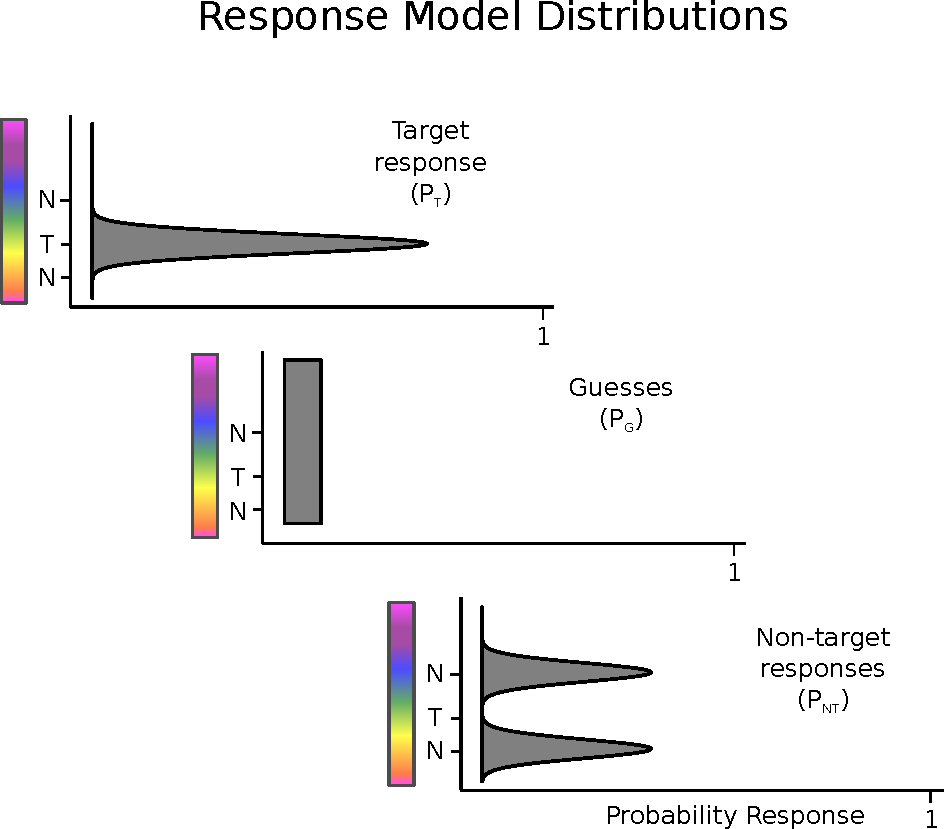
\includegraphics
	[height=.8\textheight,width=\textwidth,keepaspectratio]
	{VWM/fig_Emrich2012.pdf}
\end{frame}

\begin{frame}[noframenumbering]
	\frametitle{Figure 2.3}
	\centering
	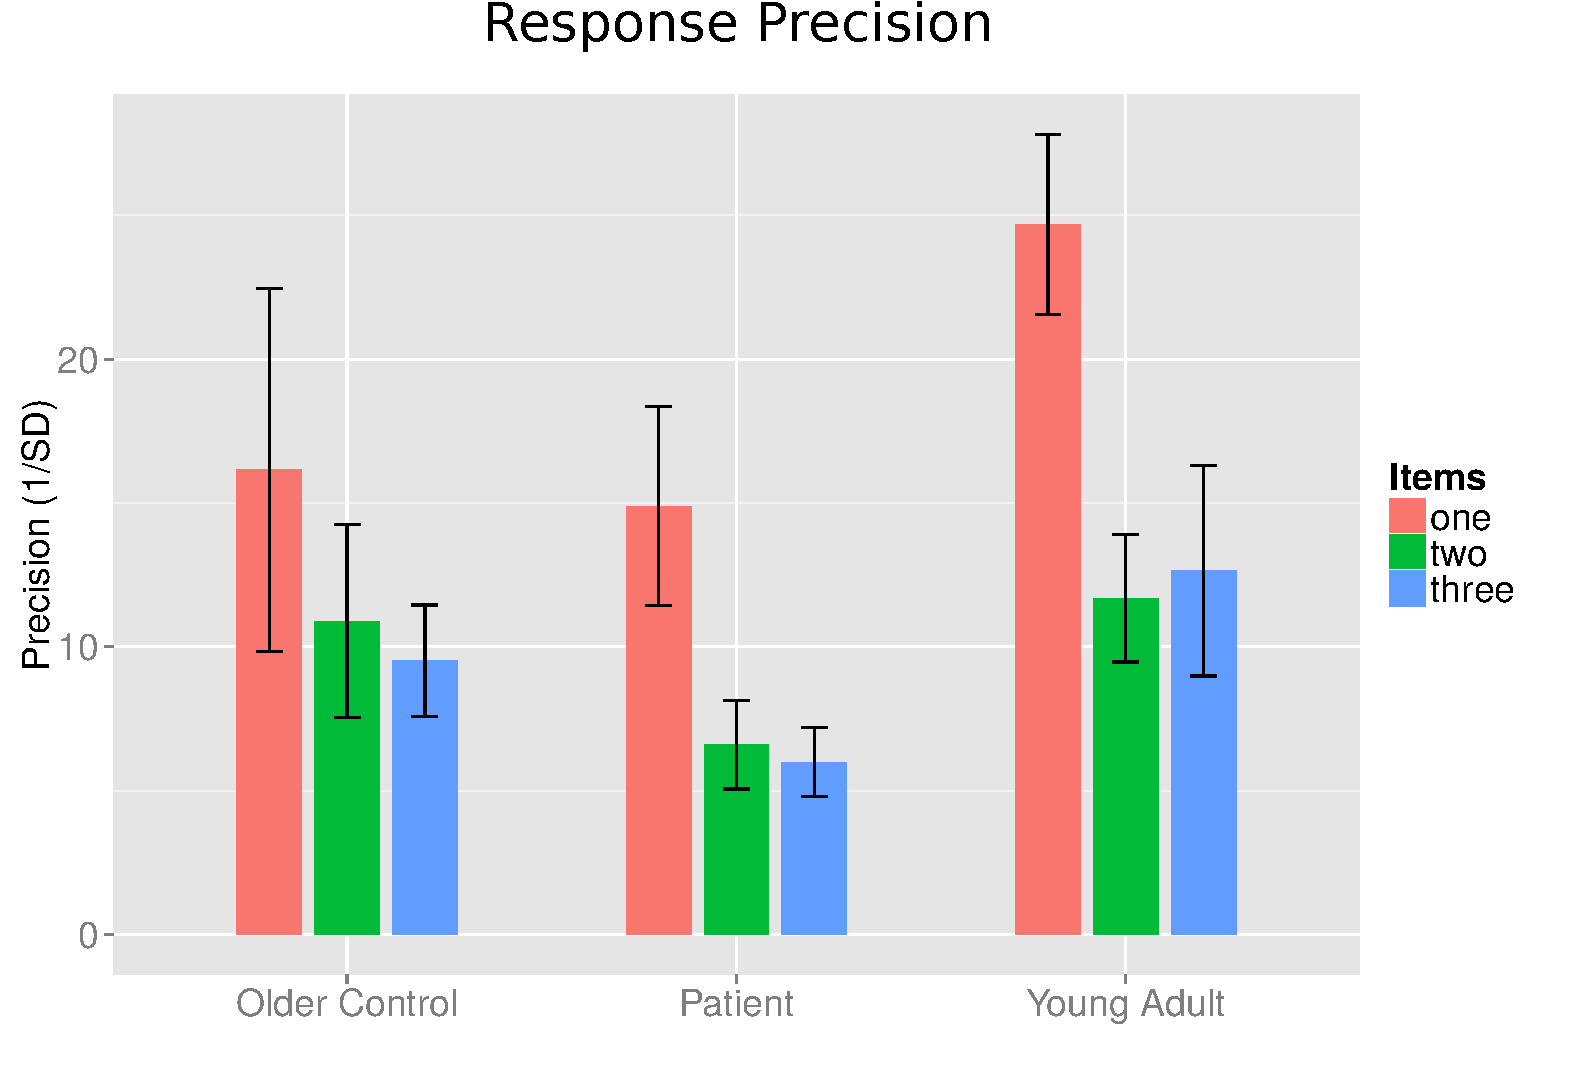
\includegraphics
	[height=.8\textheight,width=\textwidth,keepaspectratio]
	{VWM/fig_VWM_Precision.pdf}
\end{frame}

\begin{frame}[noframenumbering]
	\frametitle{Table 2.2}
	% latex table generated in R 3.1.1 by xtable 1.7-4 package
% Wed Apr 15 20:12:57 2015
\begin{table}[ht]
\centering
\begin{tabular}{lrrrrr}
  \hline
 & Df & Deviance & Resid. Df & Resid. Dev & Pr($>$Chi) \\ 
  \hline
NULL &  &  & 15 & 22.18 &  \\ 
  CES & 1 & 8.62 & 14 & 13.56 & 0.0033 \\ 
  $P_{NT}$ & 1 & 1.12 & 13 & 12.44 & 0.2908 \\ 
  $P_G$ & 1 & 12.44 & 12 & 0.00 & 0.0004 \\ 
   \hline
\end{tabular}
\caption{Analysis of deviance table. Each row represents the change in
	deviance of the model with the addition of one term. Pr($>$Chi) is the
	probability of obtaining a greater scaled deviance statistic than
	the observed under the null hypothesis (new term has true parameter of
	zero). Both CES and $P_{G}$ result in statistically significant model
	improvement.} 
\label{aod}
\end{table}

\end{frame}

\begin{frame}
	\frametitle{Experiment 2: Participants and Procedure}[noframenumbering]
\begin{itemize}
	\item 6 RBD neurological patients who demonstrated neglect in pre-testing.
	\item Line Bisection, Spatial Working Memory, and Time Estimation.
\end{itemize}
\end{frame}

\begin{frame}[noframenumbering]
	\frametitle{Table 3.1}
	\tiny
	\centering
	\setlength{\tabcolsep}{5pt}
	\begin{tabular}{rrllllllll}
  \hline
 & Age & Sex & Handedness & Star(pre) & Star(post) & Bell(pre) & Bell(post) & Copy(pre) & Copy(post) \\ 
  \hline
10 &  68 & M & Right & 93 & 87 & 100 & 89 & + & + \\ 
  27 &  43 & M & Right & 0 & 7 & 6 & 0 & - & - \\ 
  95 &  70 & M & Right & 7 & 0 & 33 & 39 & + & + \\ 
  163 &  68 & F & Left & 30 & 7 & 6 & 29 & + & + \\ 
  97 &  66 & M & Right & 0 & 0 & 0 & 0 & - & - \\ 
  171 &  71 & F & Left & 0 & 0 & 6 & 6 & + & - \\ 
   \hline
\end{tabular}

\medskip
\begin{tabular}{rrrrrrr}
	  \hline
	   & LB(pre) & LB(post) & TE(pre) & TE(post) & SWM(pre) & SWM(post) \\
	    \hline
	    10 & -0.80 & -9.90 & 0.40 & 0.40 &  &  \\
	      27 & -0.80 & 1.20 & 0.80 & 1.00 & 83.00 & 87.00 \\
	      95 & 0.30 & -3.80 & 0.40 & 0.30 & 32.00 & 35.00 \\
	      163 & 0.90 & 4.90 & 0.40 & 0.40 & 23.00 & 45.00 \\
	      97 & 1.90 & -1.60 & 0.60 & 0.60 & 43.00 & 52.00 \\
	      171 & 3.80 & 1.40 & 0.40 & 0.50 & 43.00 & 68.00 \\
	       \hline
\end{tabular}


\end{frame}

\begin{frame}[noframenumbering]
	\frametitle{Figure 3.4}
	\centering
	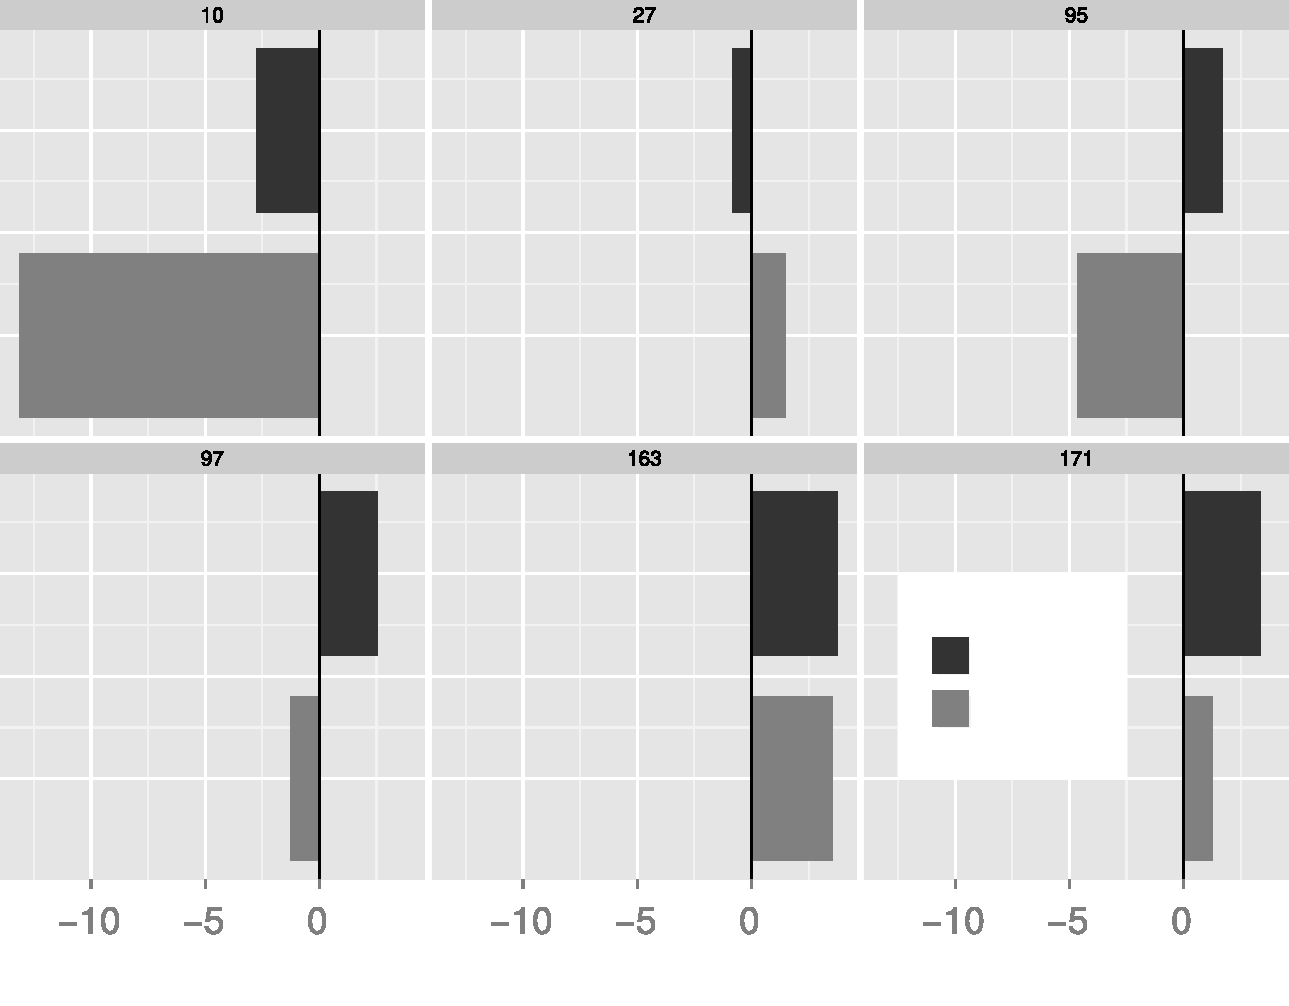
\includegraphics
	[height=.85\textheight,width=\textwidth,keepaspectratio]
	{Prisms/fig_LB_Prisms.pdf}
\end{frame}

\begin{frame}[noframenumbering]
	\frametitle{Figure 3.3}
	\centering
	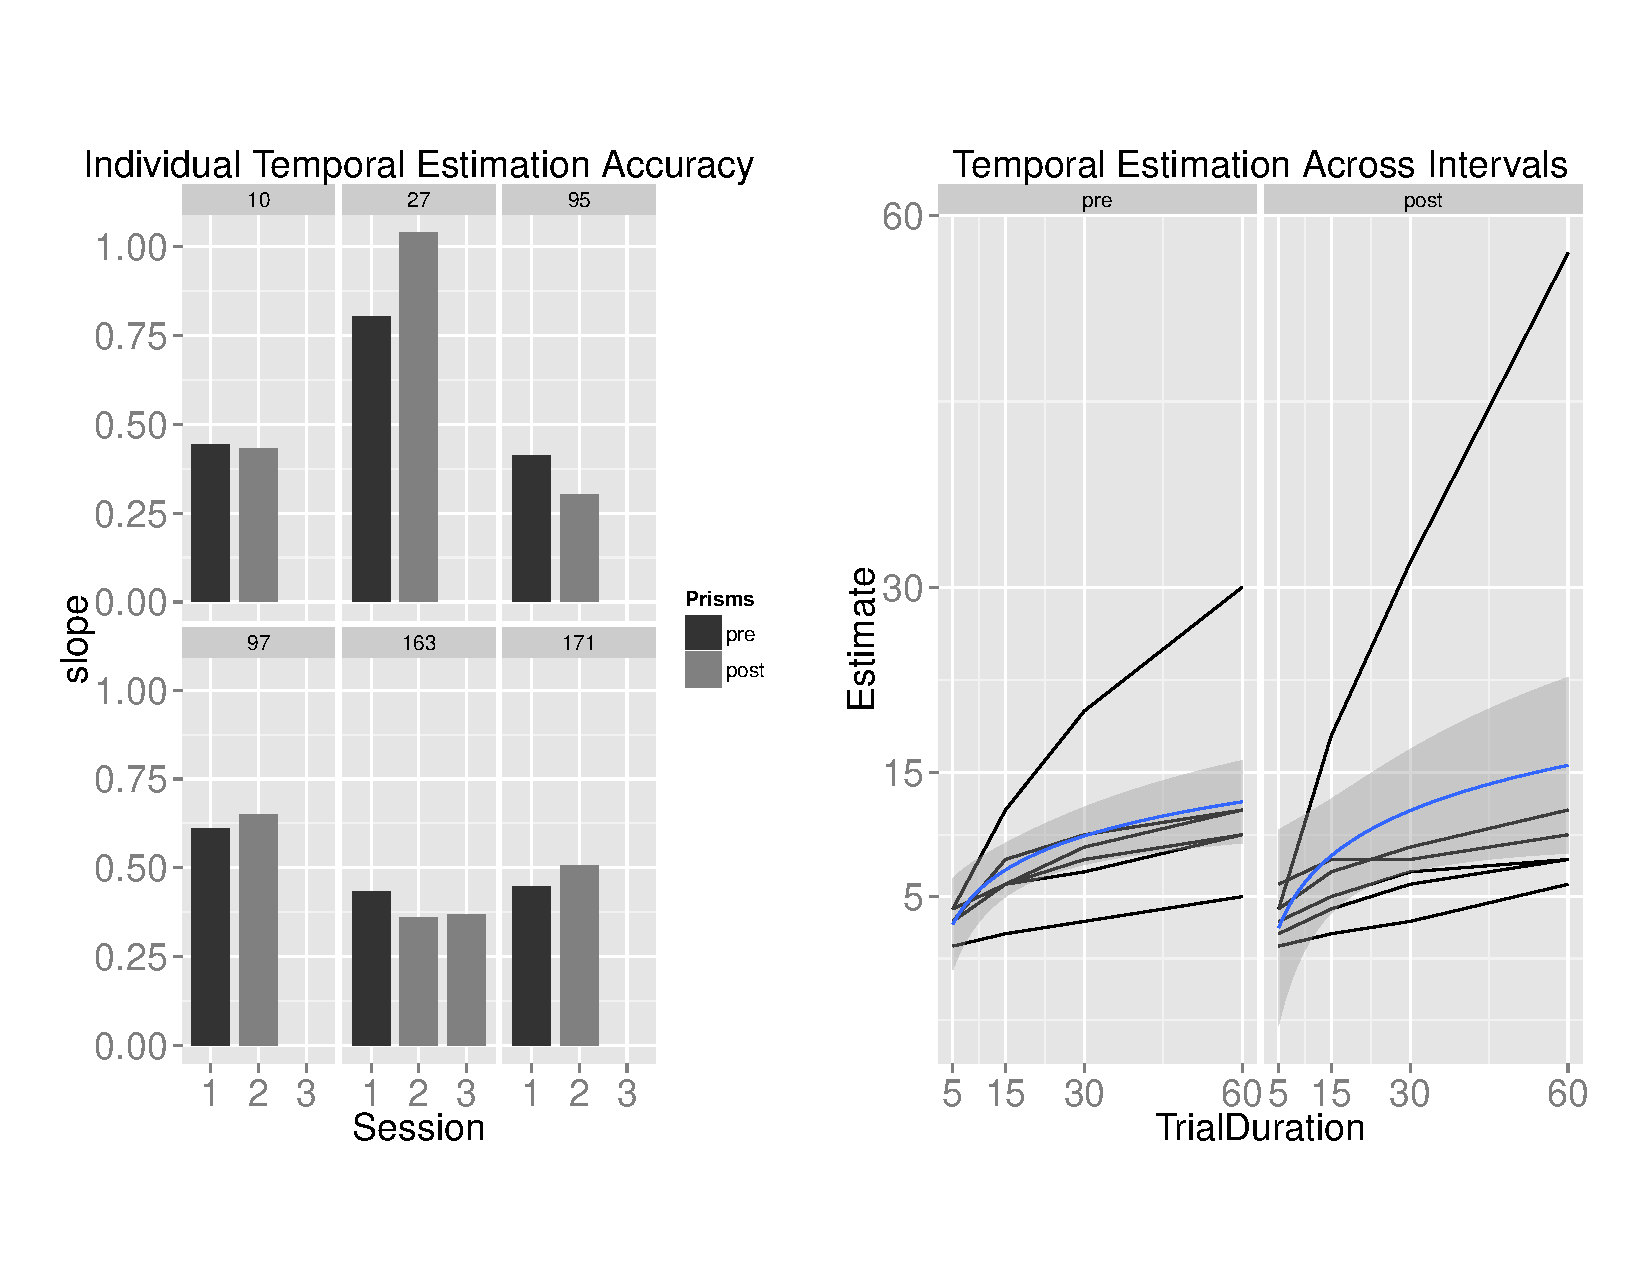
\includegraphics
	[height=.75\textheight,width=\textwidth,keepaspectratio]
	{Prisms/fig_TE.pdf}
\end{frame}

\begin{frame}[noframenumbering]
	\frametitle{Experiment 3: Participants and Procedure}
	\begin{itemize}
		\item 37 young adults.
		\item Baseline Line Bisection (LB) and Landmark Task (LT).
		\item Up to 4 blocks of Saccadic Adaptation + LB and LT.
	\end{itemize}
\end{frame}

\begin{frame}[noframenumbering]
	\frametitle{Landmark and Line Bisection Tasks}
	\centering
	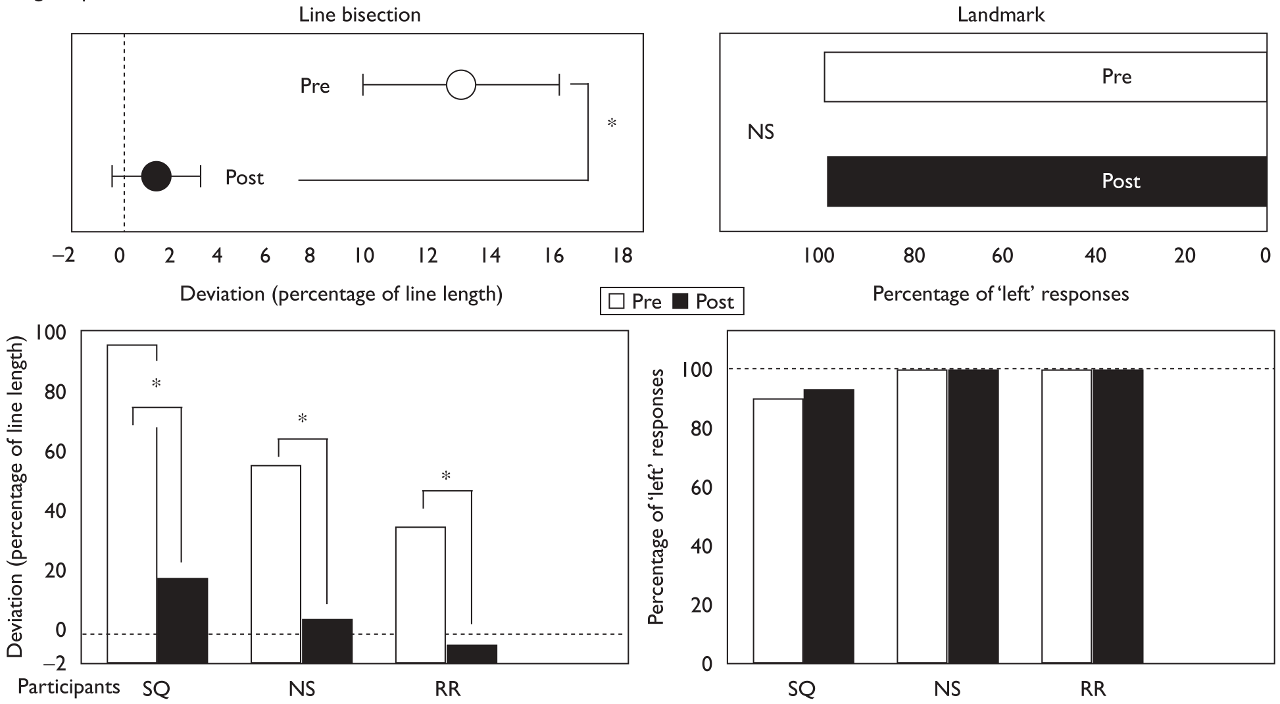
\includegraphics
	[height=\textheight,width=\textwidth,keepaspectratio]
	{img/Striemer2010.png}
	\tiny Striemer \& Danckert 2010a
\end{frame}

\begin{frame}[noframenumbering]
	\frametitle{Saccadic Adaptation Event Time-line}
	\centering
	\def\svgwidth{\textwidth}
	\tiny
	\subimport{SA/}{SA/fig_SA_b.pdf_tex}
\end{frame}


\begin{frame}[noframenumbering]
	\frametitle{Analysis of an Example Saccade}
	\centering
	\def\svgwidth{\textwidth}
	\tiny
	\subimport{SA/}{SA/fig_Saccade.pdf_tex}
\end{frame}

\begin{frame}[noframenumbering]
	\frametitle{Figure 4.4: Effect of Saccadic Adaptation}
	\centering
	\def\svgwidth{0.9\textwidth}
	\tiny
	\subimport{SA/}{SA/fig_Adaptation.pdf_tex}
\end{frame}

\begin{frame}[noframenumbering]
	\frametitle{Accepted Trials}
	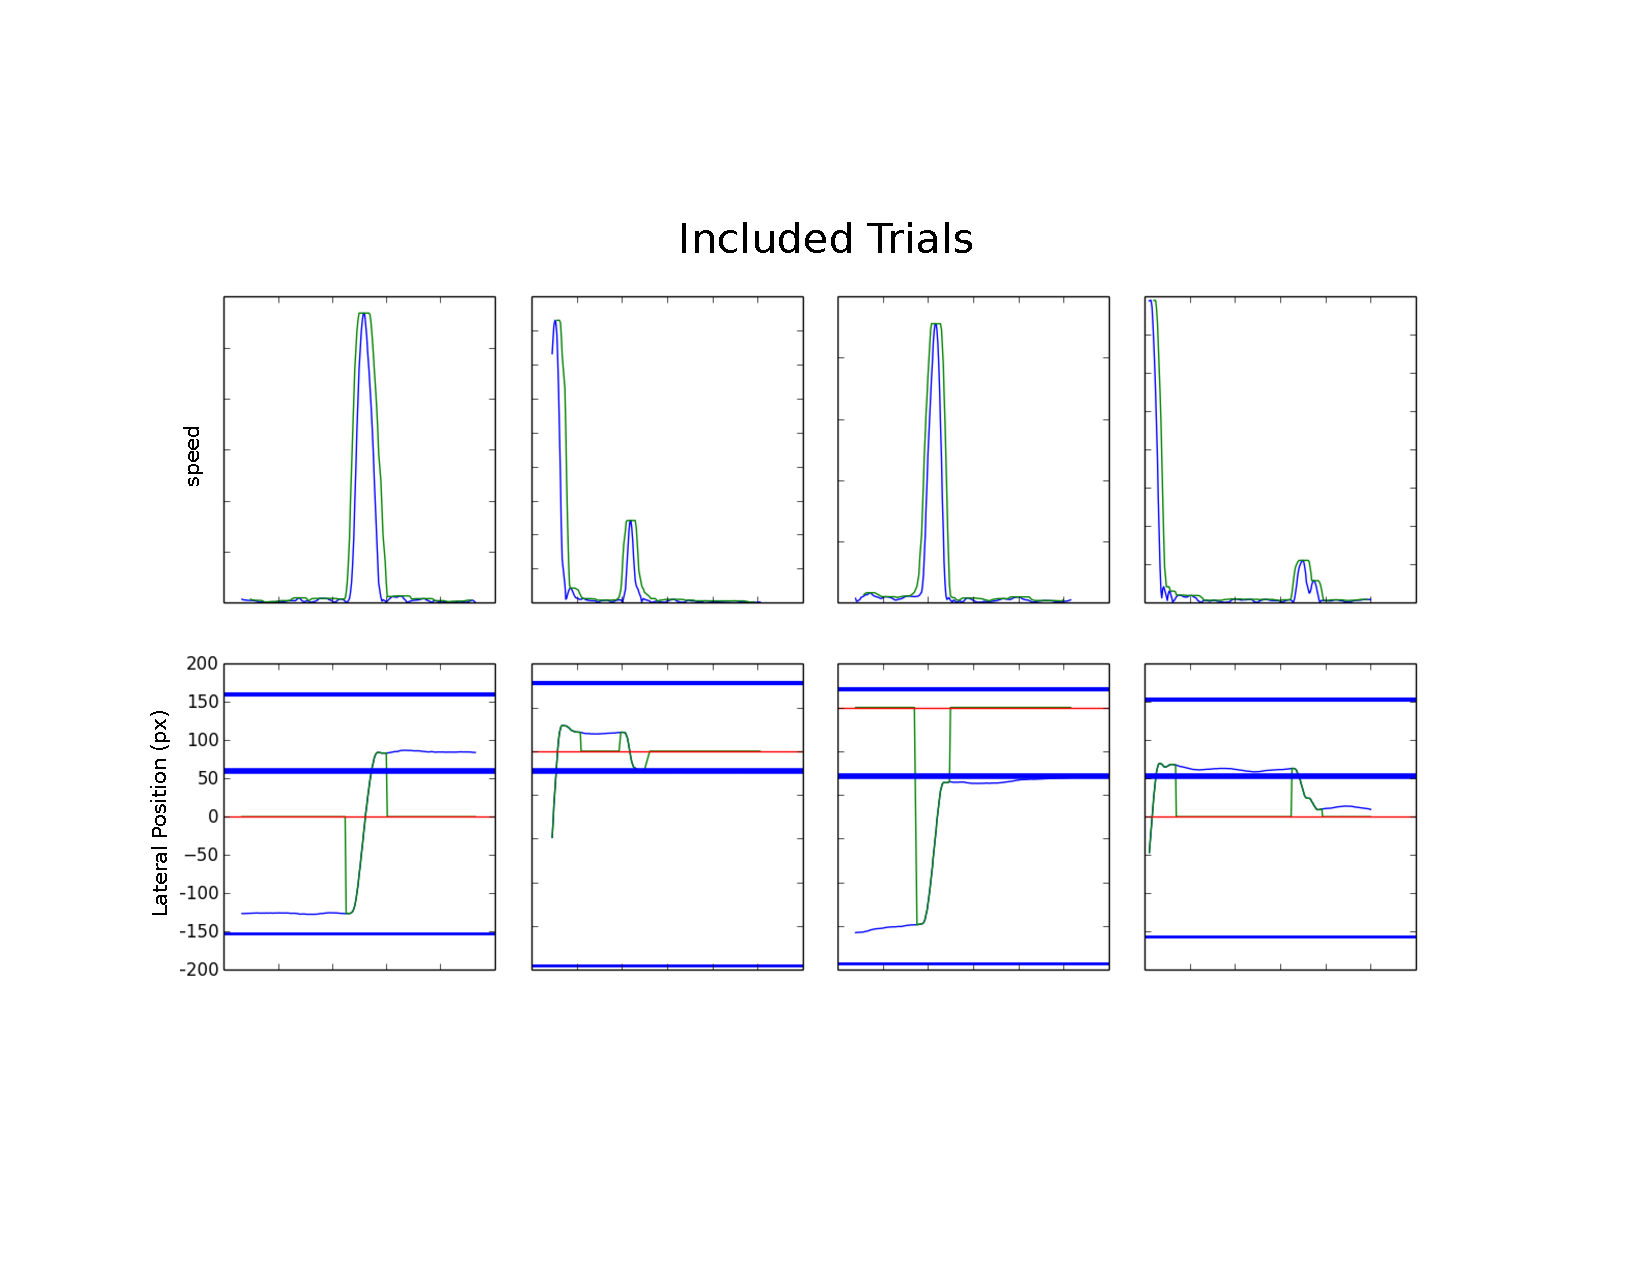
\includegraphics
	[height=1.1\textheight,width=1.1\textwidth,keepaspectratio]
	{appendix/accepted}
\end{frame}

\begin{frame}[noframenumbering]
	\frametitle{Rejected Trials}
	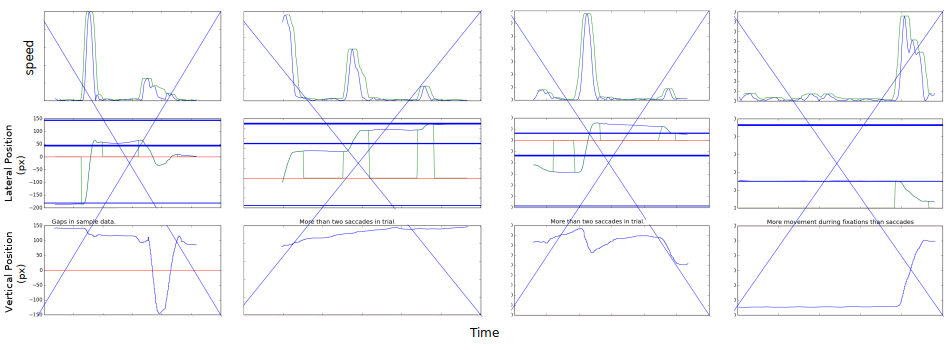
\includegraphics
	[height=1.1\textheight,width=1.1\textwidth,keepaspectratio]
	{appendix/rejected}
\end{frame}

\begin{frame}[noframenumbering]
	\frametitle{Impaired Perceptual Representation as a Key Component of Neglect}
	\begin{block}{Perceptual deficits:}
			\begin{column}{0.4\textwidth}
							\centering
							Chimeric face perception\\
							{ 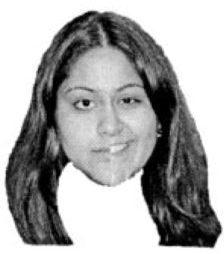
\includegraphics
							[height=.3\textheight,width=\textwidth,keepaspectratio]
							{img/chimeric.jpg}}
			\end{column}
			\begin{column}{0.6\textwidth}
							\centering
							Perceptual judgment of spatial extent.\\
							(``Landmark Task'')\\
							\smallskip
							{ 
\includegraphics
							[height=.3\textheight,width=\textwidth,keepaspectratio]
							{img/Landmark.pdf}}
			\end{column}


	\end{block}
	\begin{block}{Working Memory deficits:}
		\begin{itemize}
		\item Spatial Working Memory in Right Space.
		\end{itemize}
	\end{block}
\end{frame}
\end{document}
